\section{Metode}
\noindent\textbf{Utstyr}:
\begin{itemize}
    \item Telefon
    \item Telefonholder
    \item Trefot
    \item Vater
\end{itemize}

\subsection{Valg av referansepunkter og målelokasjon}
Det ble gjort målinger ved 2 referansepunkt for å bedre datagrunnlag. Koordinatene til $B$ og $C$ blir estimert ved hjelp av Google Maps. Koordinatene til målelokasjonen $A$ ble målt ved hjelp av Phyphox \cite{phyphox}. $\theta_1$ og $\theta_2$ er vinklene mellom hhv. spiret på Nidarosdomen og geografisk nord, og mellom Tyholttårnet og geografisk nord.


\subsection{Måling av magnetfelt og oppsett}
En trefot ble brukt med en plattform for telefonene, hvor telefonene ble plassert i en telefonholder. For å gi riktig retning på telefonene, ble det plassert ett vater langsmed telefonholderen \ref{fig:med_vater}. Referansepunktene som ble brukt Vateret ble så brukt som siktemiddel slik at telefonholderen, og dermed telefonen lå i retning av referansepunktet som ble siktet på. Deretter ble plattformen justert slik at den var horisontal ved hjelp av et vater.

Før hver måling ble telefonene kalibrert ved å spinne de rundt. Deretter ble telefonene plassert i telefonholderen og ble liggende der en tid til målingene var stabile. Dataene ble så eksportert. 

Det ble gjort måling om flymodus og restarting av telefonene ville ha effekt. Disse målingen ble gjennomført med telefonene pekende mot Tyholttårnet. Målingene med flymodus ble gjennomført ved at telefonene ble satt i flymodus, kalibrert og dermed satt i telefonholderen. Målingene med restarting ble gjennomført ved at telefonene ble restartet, kalibrert og så plassert i telefonholderen.

For å finne posisjonen til målepunktet ble phyphox benyttet. Da med «Location» som måling for GPS-koordinater. Telefonene ble kalibrert ved at de ble beveget noen meter i ulike retninger før selve målingen ble utført i telefonholderen. Målingene ble utført på vestre siden av broen som krysser Eidsvolls gate langs Øvre alle. 
For å finne koordinater for Nidarosdomen og Tyholttårnet ble Google Maps brukt.
Dataene ble så analysert i Python ved hjelp av teorien beskrevet ovenfor, for å finne gjennomsnittsverdi, median og standardavvik for deklinasjonen og inklinasjonen for hver måleserie.     

 
\begin{figure}
    \centering
    \includegraphics[width=0.45\textwidth]{img/Plattform med vater.pdf}                 
    \caption{Figuren viser oppsettet for måling før telefonen ble plassert i telefonholderen. Vateret er siktemiddel for referansepunktet.
        }
    \label{fig:med_vater}
\end{figure} 